\section{Udvælgelse af gestik-par til at skifte musiknummer}
\label{TestresultaterSkiftMusiknummer}
%
Udvælgelsen af hvilket gestik-par, der skal knyttes til at skifte musiknummer foretages på baggrund af testpersonernes begrundelser for til- og fravalg af de foreslåede gestikker. Der fokuseres først på hvilke gestik-par testpersonerne har inddraget i deres top tre rangering og i den forbindelse, om det er muligt at ekskludere nogle gestik-par. Derefter fokuseres der på testpersonernes begrundelser for, hvorfor de har valgt de gestik-par, som de har, hvorunder forbedringsforslag inkluderes, hvis testpersonerne fremsætter nogle. Afsnittet vil afslutningsvist ende ud i hvilket gestik-par, der vælges til at skifte musiknummer.\blankline
%
Få at få et overblik over, hvor ofte de syv forskellige gestik-par individuelt indgår på enten en første-, anden- eller tredjeplads i top tre rangeringen opstilles følgende \autoref{fig:SamletTopTreSkift}. 
%
\begin{figure}[H]
	\centering
	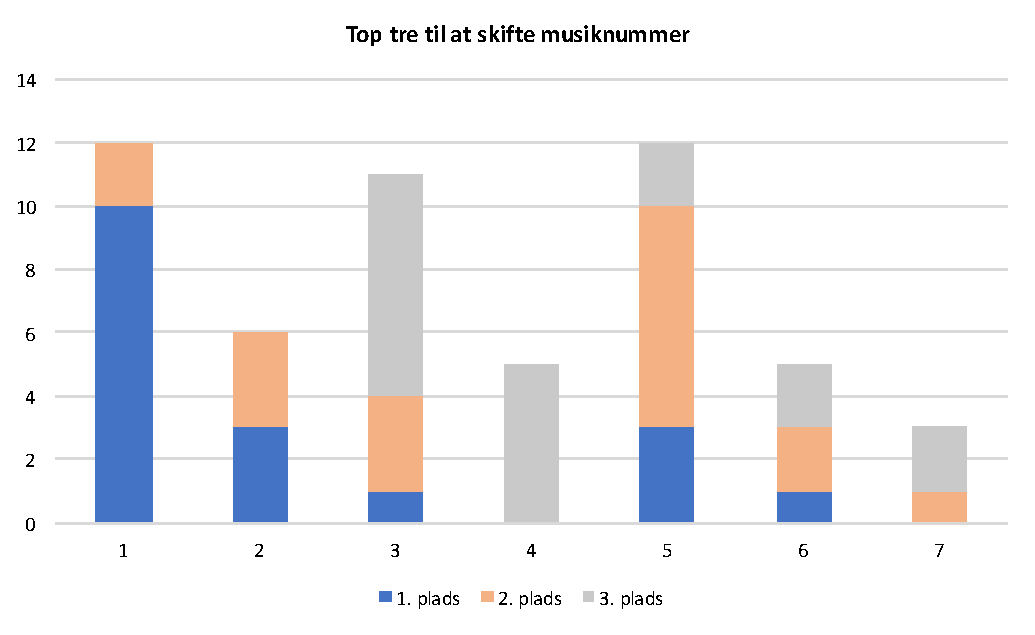
\includegraphics[resolution=300,width=0.9\textwidth]{Test1/DatabehandlingGrafer/TopTreSkift}
	\caption{Søjlediagram over hvordan hvert gestik-par indgår i testpersonernes top tre i forhold til at skifte musiknummer. Data forefindes i \autoref{app:TopTreRangeringSkift}.}
	\label{fig:SamletTopTreSkift}
\end{figure}
\noindent
%
På \autoref{fig:SamletTopTreSkift} fremgår det tydeligt, at GP1, GP3 samt GP5 er de tre gestik-par, som uafhængigt af den specifikke plads, indgår flest gange i testpersonernes top tre. Derudover tyder det på, at hverken GP4, GP6 eller GP7 er specielt eftertragtet, da de henholdvis kun indgår fem, fem og tre gange i testpersonernes samlede top tre, jævnfør \autoref{fig:SamletTopTreSkift}. For at vurdere om der er belæg for, at ekskludere et eller flere gestik-par opstilles følgende \autoref{fig:DaarligstGestikSkift}. 
%
\begin{figure}[H]
	\centering
	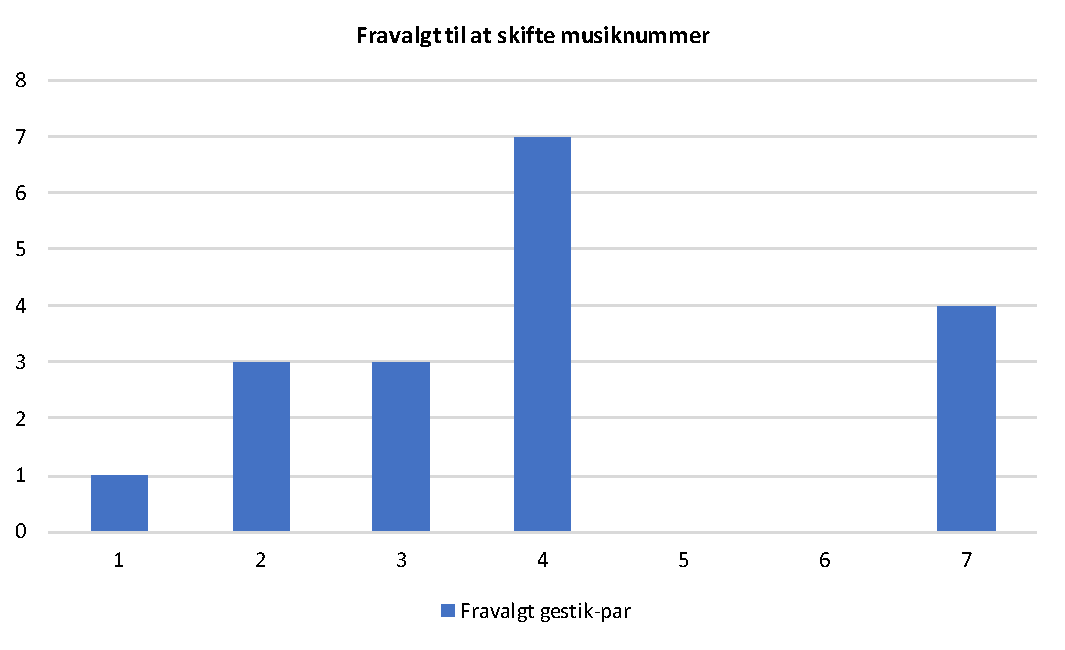
\includegraphics[resolution=300,width=0.9\textwidth]{Test1/DatabehandlingGrafer/FravalgtSkift}
	\caption{Søjlediagram over hvilke gestik-par testpersonerne fravælger i forbindelse med at skifte musiknummer.}
	\label{fig:DaarligstGestikSkift}
\end{figure}
\noindent
%
På \autoref{fig:DaarligstGestikSkift} opsummeres antallet af gange hvert gestik-par fravælges af testpersonerne. Da syv ud af 18 testpersoner har fravalgt GP4 konkluderes det, at testpersonerne ikke bryder sig om GP4, hvorfor GP4 ekskluderes. På \autoref{fig:SamletTopTreSkift} fremgår det, at GP6 kun tildeles én førsteplads og derudover kun indgår to gange på henholdvis en anden- og tredjeplads og selvom GP6 aldrig fravælges af testpersonerne, så vurderes det, at GP6 er overflødig og irrelevant. Der er derfor belæg for at ekskludere GP6. Tilsvarende er gældende for GP7, som kun indgår tre gange i testpersonernes samlede top tre og aldrig tildeles en førsteplads, jævnfør \autoref{fig:SamletTopTreSkift}, og derudover fravælges fire gange, jævnfør \autoref{fig:DaarligstGestikSkift}. Der er derfor belæg for at ekskludere GP7. Selvom GP2 indgår seks gange i den samlede top tre, så ekskluderes dette gestik-par. Det gøres, blandt andet, ud fra et ønske om ikke at gå i mod Bang $\&$ Olufsen's designvalg i forhold til, hvilken retning swipe-bevægelsen skal foretages i for at skifte til det næste musiknummer. I \autoref{app:TestresultaterSkiftDaarlig} forefindes en dybere analyse af hvorfor testpersonerne fravælger de gestik-par, som de gør. 

Ekskluderingen af de fire gestik-par medfører, at den efterfølgende analyse vil omhandle testpersonernes begrundelser for at vælge GP1, GP3 samt GP5.
%
\subsection{Testpersonernes begrundelse for valg af gestik-par 1}
\label{TestresultaterValgAfGestikkerBegrundelseGP1Skift}
%
Med udgangspunkt i \autoref{fig:SamletTopTreSkift} tildeles GP1 en førsteplads af 10 testpersoner, en andenplads af to testpersoner og aldrig en tredjeplads. GP1 illustreres på \autoref{fig:GestikPar1Skift}. De testpersoner, som har tildelt GP1 en førsteplads, begrunder det ud fra en kombination af følgende egenskaber: 
%
\begin{multicols}{3}
    \begin{itemize}
        \item Foretrækker dynamik
        \item Naturlig
        \item Giver mening
        \item Simpel
        \item Intuitiv
        \item Logisk
        \item Enkel
        \item Nem at udføre
        \item Nem at forstå
\end{itemize}
\end{multicols}
\noindent
%
Derudover relaterer testpersonerne GP1 til hvordan der normaltvist interageres med tablets og smartphones, hvilket indikerer at de har erfaring med swipe-bevægelser. Ydermere påpeges det, at der i GP1 ikke er et besværligt håndtegn, som skal gengives for at skifte musiknummer.
%
\begin{figure}[H]
	\centering
	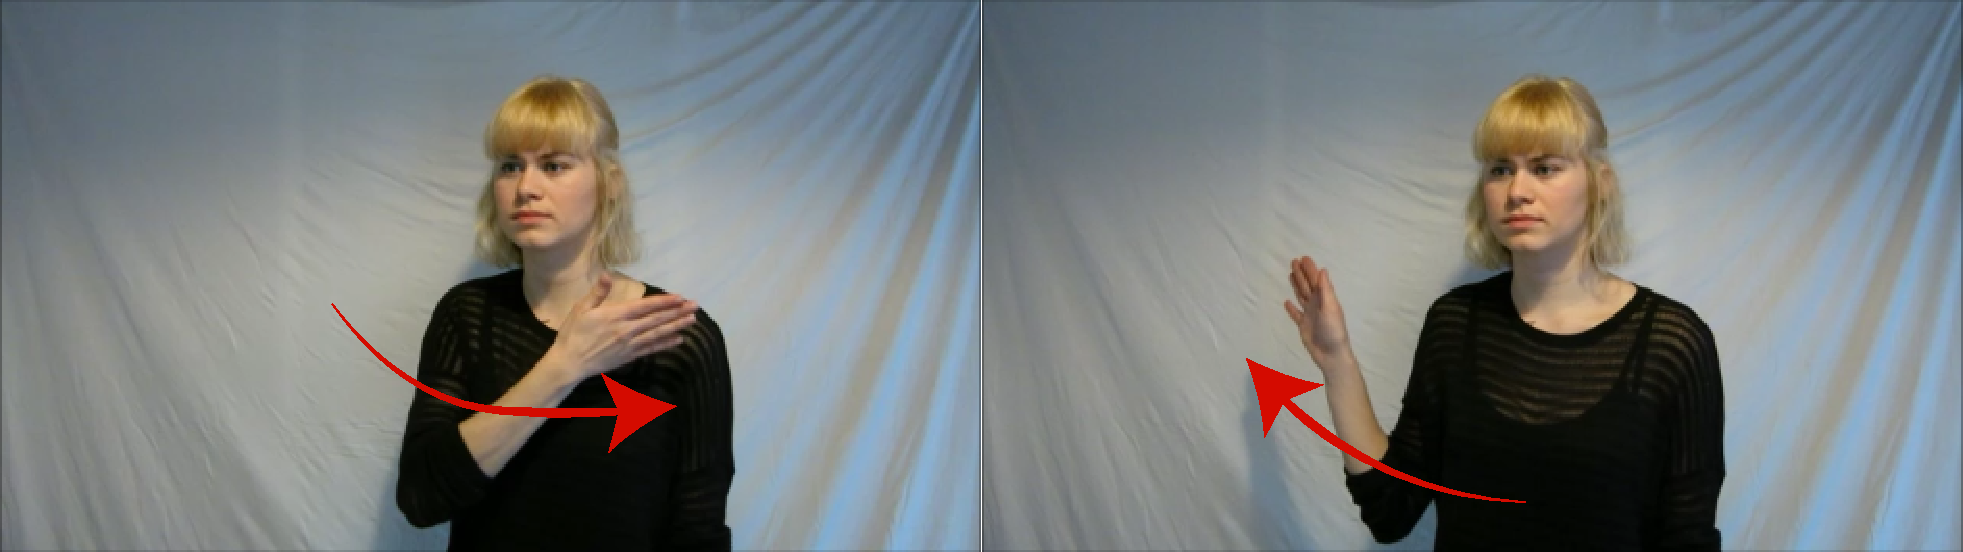
\includegraphics[resolution=300,width=0.9\textwidth]{Test1/Gestik-par/Gestik1_SkiftSang}
	\caption{Illustration af gestik-par 1; swipe fra højre mod venstre for at skifte til det næste musiknummer og fra venstre mod højre for at skifte til det forrige musiknummer.}
	\label{fig:GestikPar1Skift}
\end{figure}
\noindent
%
Sammenholdes udtalelserne fra de 10 testpersoner med hvad de rent faktisk gør så er der fire, som ikke formår at udføre bevægelsen i GP1 konsekvent. TP1 alternerer mellem at gengive GP1 og GP5 når testpersonen generelt referer til en swipe-bevægelse, men når testpersonen afslutningsvist gengiver sine fortrukne gestikker, så gengives GP1. I \autoref{app:VideooptagelseValgAfGestikkerTestpersoner} forefindes videomaterialet for den pågældende situation. I begyndelsen foretrækker TP7 GP7, hvorefter testpersonen ræsonnerer sig frem til, at det istedet er GP1 testpersonen foretrækker. Dog med forbehold for at TP7 foretrækker en mindre bevægelse. Når TP7 afslutningsvist gengiver sine fortrukne gestikker, så gengives GP5, dog i den modsatte retning. Når TP15 taler om GP2, så gengiver testpersonen GP1 og når testpersonen opfordres til at prøve gestikkerne til musik så gengives de med både højre og venstre hånd, hvor begge bevægelser er modsat af bevægelsen i GP1. Afslutningsvist er det dog GP1, som TP15 gengiver. Samme tendens forefindes ved TP16, som først gengiver GP1, hvorefter der afslutningsvist forklares og gengives bevægelsen svarende til GP2. Testlederen gengiver GP1 for, at være sikker på hvad TP16 foretrækker, hvor testpersonen giver udtryk for, at det er sådan det skal være. I begge tilfælde, så er der indikationer af, at både TP15 og TP16 er i tvivl om hvilken retning swipe-bevægelsen skal foregå i for at skifte til enten det næste eller forrige musiknummer.

Derudover påpeger TP6 et potentielt problem, som opstår når der skal skiftes tilbage til det forrige musiknummer og ikke for at genspille musiknummeret. Testpersonen er bekymret for, at det bliver nødvendigt at svinge mange gange i luften, for at rent faktisk at skifte til det forrige musiknummer. Det er selvfølgelig en problemstilling, der skal tages højde for, men som det er kendt fra andre musikafspillere; så skiftes der til det forrige musiknummer, hvis det gøres inden for relativt kort tid, derefter genspilles musiknummeret. Det antages derfor at dette ligeledes implementeres i Bang $\&$ Olufsen's fremtidige musikanlæg. 
%
\subsubsection{Forbedringsforslag til gestik-par 1}
\label{TestresultaterValgAfGestikkerForbedringGP1Skift}
%
Af de 10 testpersoner, som har valgt GP1, er der fire testpersoner, som har forbedringsforslag. Ifølge TP2 skal antallet af fingre i swipe-bevægelsen være ligegyldig, da det er bevægelsen, der er essentiel. Det antages derfor at testpersonen formentlig ikke vil have noget imod at benytte GP5 istedet. Testpersonen har tildelt GP5 en andenplads. TP5 foreslår at bevægelsen skal være et "ninja hug", hvor fingrene samles, håndfladen peger opad og bevæges skråt ned fra højre mod venstre for at skifte til det næste musiknummer. For at skifte til det forrige musiknummer, foreslår TP5, igen at fingrene samles med denne gang skal håndfladen pege nedad og bevæges skråt ned fra venstre mod højre. Forbedringsforslaget afvises dog, da bevægelsen bliver stiv og bestemt, hvilket forventes at have en negativ effekt på den sociale accept.

For at undgå det problem, som TP6 påpeger, foreslår testpersonen at GP3 benyttes til at skifte til det forrige musiknummer, for at undgå genspilningen. Dette forslag afvises dog, da en opdeling af funktionen potentielt kan gøre det svære at lærer og derudover afviger det fra hvordan tilbage-funktionen normalvist fungerer. 

For at skifte til det næste musiknummer foreslår TP10, at højre hånd føres ind foran kroppen og for at skifte til det forrige musiknummer føres venstre hånd ind foran kroppen. Uanset om det er GP1 eller andre, der anvendes til at skifte musiknummer, så forventes det, at det er muligt at gengive gestikken med begge hænder. Det er derfor uhensigtmæssigt at knytte en bestemt hånd til en bestem retning, hvorfor forbedringsforslaget afvises.     
%
\subsection{Testpersonernes begrundelse for valg af gestik-par 3}
\label{TestresultaterValgAfGestikkerBegrundelseGP3Skift}
% 
Med udgangspunkt i \autoref{fig:SamletTopTreSkift} tildeles GP3 en førsteplads af én testperson, en andenplads af tre testpersoner og en tredjeplads af syv testpersoner. GP3 illustreres på \autoref{fig:GestikPar3Skift}. 

Årsagen til at TP8 har tildelt GP3 en førsteplads er, fordi det er klart og tydeligt hvad der skal gøres. Foruden GP3 så har TP8 tildelt GP7 en tredjeplads, jævnfør \autoref{app:TopTreRangeringSkift}, hvilket indikerer at testpersonen foretrækker en lille bevægelsesmængde. Da der kun er én enkelt testperson, som har tildelt GP3 en førsteplads vælges det, at inddrage responsen fra de testpersoner, som tildelte GP3 en anden- eller tredjeplads. De testpersoner, som har tildelt GP3 en anden- eller tredjeplads, begrunder det ud fra en kombination af følgende egenskaber: 
%
\begin{multicols}{3}
    \begin{itemize}
        \item Diskret
        \item Nem at udføre
        \item Nem at overse
        \item Statisk
        \item Simpel
        \item Passiv
\end{itemize}
\end{multicols}
\noindent
%
TP2 og TP5 inkluderer kun GP3 fordi de enten ikke accepterede de andre foreslag eller fordi det var det gestik-par, som kom tættest på en tredjeplads. Ligende tendens forefindes ved TP9, som benytter udelukkelsesmetoden til at danne sin top tre.
%
\begin{figure}[H]
	\centering
	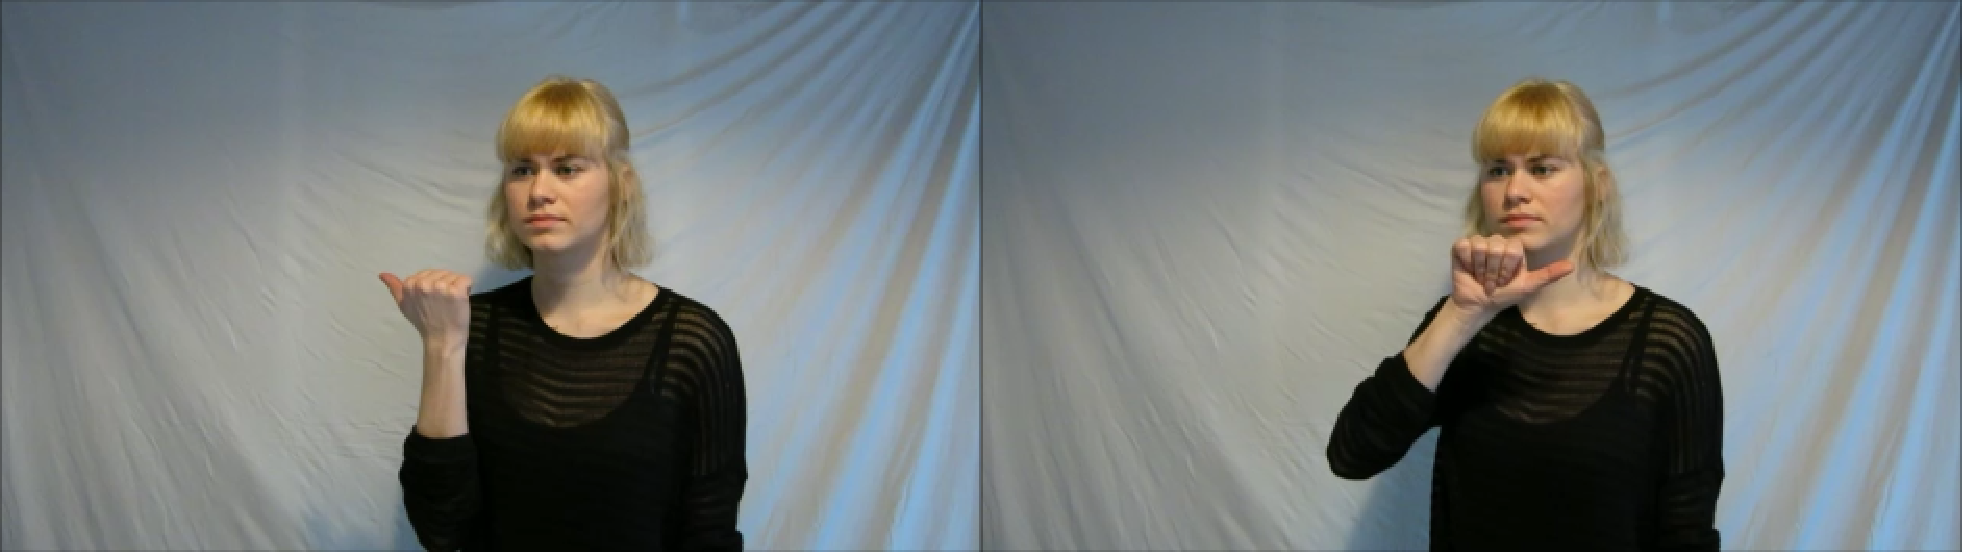
\includegraphics[resolution=300,width=0.9\textwidth]{Test1/Gestik-par/Gestik3_SkiftSang}
	\caption{Illustration af gestik-par 3; tommelfinger peger den retning musiknummeret skal skifte i. Først frem og derefter tilbage til det forrige musiknummer.}
	\label{fig:GestikPar3Skift}
\end{figure}
\noindent
% 
Da der kun er én enkelt testperson, som har tildelt GP3 en førsteplads og at det derudover tyder på, at GP3 kun indgår fordi testpersonerne har benyttet udelukkelsesmetoden, så vurderes det, at der belæg for at ekskludere GP3.
%
\subsection{Testpersonernes begrundelse for valg af gestik-par 5}
\label{TestresultaterValgAfGestikkerBegrundelseGP5Skift}
%
Med udgangspunkt i \autoref{fig:SamletTopTreSkift} tildeles GP5 en førsteplads af tre testpersoner, en andenplads af syv testpersoner og en tredjeplads af to testpersoner. GP5 illustreres på \autoref{fig:GestikPar3Skift}. De testpersoner, som har tildelt GP5 en førsteplads, begrunder det ud fra en kombination af følgende egenskaber: 
%
\begin{multicols}{3}
    \begin{itemize}
        \item Nem at huske
        \item Elegant
        \item Logisk
        \item Intuitiv
        \item Giver god mening
\end{itemize}
\end{multicols}
\noindent
%
Derudover giver TP11 udtryk for, at de gestik-par, som indgår i top tre rangeringen vælges ud fra hvad der mindst naturligt i en samtale, hvorfor testpersonen har tildelt GP5 en førsteplads. Lignende tendens forefindes ved TP14, som konsekvent vælger gestikker efter hvad der føles unaturligt og som testpersonen ikke fejlagtigt kommer til at gengive i en samtale. Derudover giver TP14 udtryk for at et bestemt håndtegn er at foretrække. Det skal dog pointeres, at både TP11 og TP14 foretrækker, at gestikkerne er unaturlige, hvilket i deres tilfælde forbindes med noget positivt. Dog forbinder TP14 GP5 med en swipe-bevægelsen, hvilket testpersonen finder naturligt.  
%
\begin{figure}[H]
	\centering
	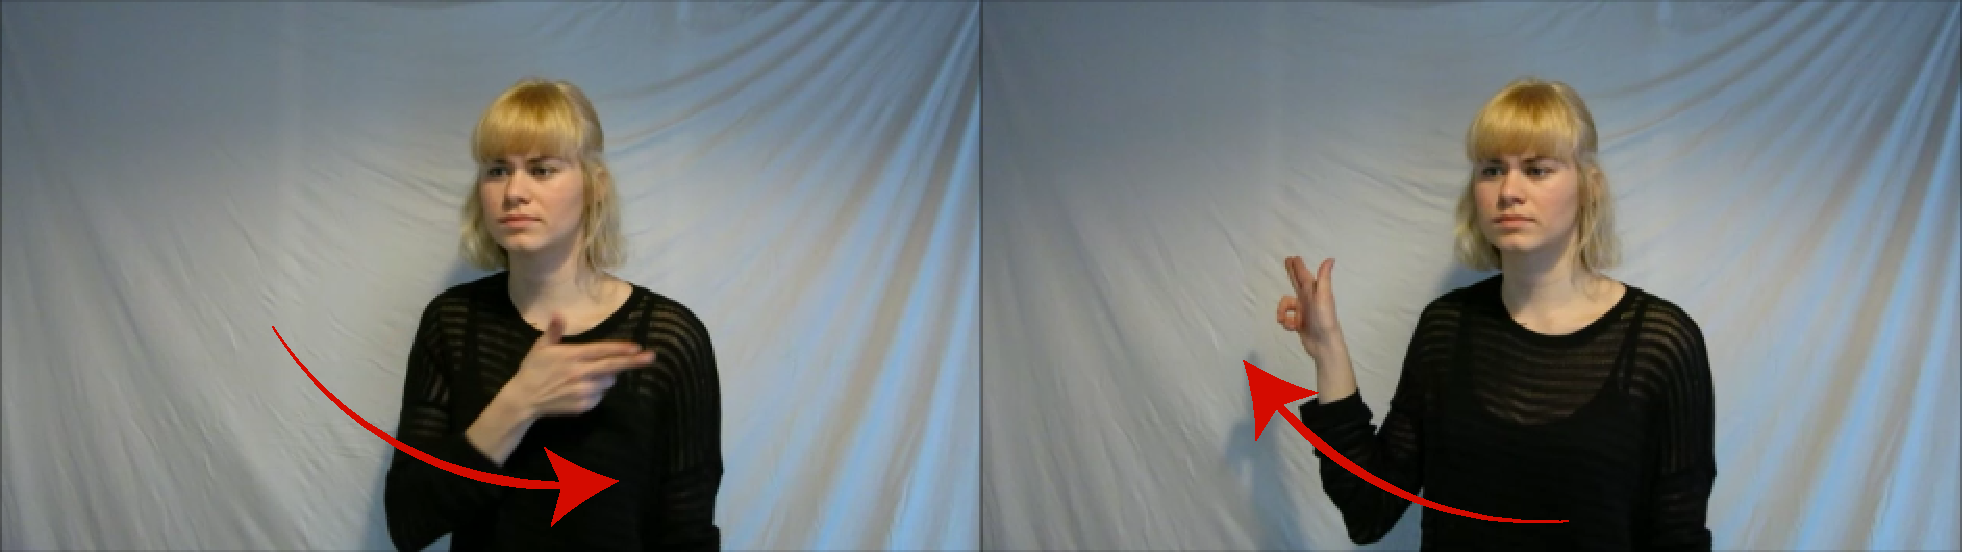
\includegraphics[resolution=300,width=0.9\textwidth]{Test1/Gestik-par/Gestik5_SkiftSang}
	\caption{Illustration af gestik-par 5; swipe med pege- og langefinger fra højre mod venstre for at skifte til det næste musiknummer og fra venstre mod højre for at skifte til det forrige musiknummer.}
	\label{fig:GestikPar5Skift}
\end{figure}
\noindent
%
Selvom GP5 kun tildeles en førsteplads tre gange, så indgår GP5 i testpersonernes samlede top tre ligeså ofte, som GP1, jævnfør \autoref{fig:SamletTopTreSkift}. Det vælges derfor, at inddrage responsen fra de testpersoner, som tildelte GP3 enten en anden- eller tredjeplads.\blankline
%
Den gennemgående tendens er, at når testpersonerne tildeler GP5 en andenplads, så skyldes det, at GP5 minder mest om GP1, som af tre testpersoner tildeles førstepladsen. Med forbehold for, at TP4 tildeler GP2 førstepladsen, så tildeles GP5 andenpladsen af samme årsag; GP5 minder mest om GP2, hvis bevægelsesretningen i GP5 ændres derefter. 

Lignende tendens forefindes ved TP13, som tildeler GP5 andenpladsen fordi GP5 er næstmest naturlig sammenlignet med GP1. Dog kommenterer testpersonen, at det giver bedre mening at benytte to fingre til at flytte på noget, hvilket TP5 ligeledes giver udtryk for, som i tillæg kommenterer at to fingre tillader kontrol over det der skubbes til. Derudover tilføjer TP5 at GP5 er mindre voldsom og nemmere at udføre siddende sammenlignet med GP1. TP13 giver udtryk for at foretrække gestikker, som dels kræver en bevægelse og dels er defineret ud fra et bestemt håndtegn, hvilket formentligt er årsagen til at GP1 ikke fremgår i testpersonens top tre, jævnfør \autoref{app:TopTreRangeringSkift}.

Af de 12 gange GP15 indgår i en top tre, så er der fire testpersonerne, som har undladt GP1. Fokuseres der på hvad de fire testpersoner ellers har inkluderet i deres top tre, så er det kun TP4, som inkluderer et statisk gestik-par; GP3. De tre resterende testpersoner inkluderer gestik-par, som består af en swipe-bevægelse, jævnfør \autoref{app:TopTreRangeringSkift}. Sammenlagt er der fem ud af 12 testpersoner, som foruden at inkludere GP5 i deres top tre, inkluderer GP3. Dog rangeres GP5 altid højere end GP3.\blankline 
%
Den generelle tendens er, at testpersonerne i høj grad foretrækker at gengive dynamiske gestikker for at skifte musiknummer. Særligt en swipe-bevægelse, som forbindes med interaktionen på en tablet eller en smartphone, foretrækkes. Derudover er den største årsag til at GP5 tildeles en andenplads fordi den minder mest om GP1.   
%
\subsubsection{Forbedringsforslag til gestik-par 5}
\label{TestresultaterValgAfGestikkerForbedringGP5Skift}
%
Af de tre testpersoner, som har valgt GP5, er der to testpersoner, som har forbedringsforslag. TP9 foreslår at bevægelsen gengives med tre fingre, for at undgå et pistolagtigt udtryk. Problemet med at gengive GP5 med tre fingre er, at det kan være svært og ubehageligt at strække ringefingeren samtidig med at lillefingeren bøjes, hvilket er årsagen til at forbedringsforslaget afvises. Forbedringsforslaget fremsat af TP11 anses for at være en selvfølge; forbedringen, ifølge TP11, er at bevægelsesmængden reduceres så det eksempelvis er muligt at skifte musiknummer med en swipe-bevægelse direkte fra håndleddet. 
%
\subsection{Valg af gestik-par til at skifte musiknummer}
\label{TestresultaterValgAfGestikkerValgSkift}
%
Baseret på foregående analyse samt \fullref{app:TestresultaterSkiftDaarlig} hvor i alt fem gestik-par er ekskluderet, så står valget mellem GP1 og GP5. Fælles for de to gestik-par er, at de indgår lige mange gange i testpersonernes samlede top tre; 12 gange i alt, det til trods for at GP1 indgår på en førsteplads 10 gange, hvor GP5 kun indgår på en førsteplads tre gange. Baseret på responsen fra de testpersoner, som har rangeret GP1 højere end GP5, så tyder det på, at der ikke er så stor forskel mellem de to gestik-par fordi de minder meget om hinanden.

Derudover pointerer flere testpersoner, som ikke nødvendigvis har rangeret GP1 over GP5, at de foretrækker dels, at gestikken er dynamisk og dels, at der er knyttet et bestemt håndtegn til gestikken. Ydermere er der flere testpersoner, som begår fejl når de udfører GP1, hvorimod ingen testpersoner begår fejl når de udfører GP5. Endvidere påpeger flere testpersoner at bevægelsen i GP1 er naturlig, hvorfor det antages at bevægelsen formentlig forekommer ubevidst i deres kropssprog. I tillæg vurderes det, at størstedelen af de egenskaber testpersonerne foretrækker ved GP1 går igen ved GP5. Med alt taget i betragtning vurderes det, at der er belæg for at knytte GP5 til at skifte musiknummer.
